\documentclass[a4paper,12pt]{article}

% Required packages
\usepackage{amsmath,amssymb,amsthm}
\usepackage[linesnumbered,ruled,vlined]{algorithm2e}
\usepackage{tikz}
\usetikzlibrary{arrows,positioning}
\usepackage[margin=2cm]{geometry}
\usepackage{graphicx}
\usepackage{caption}
\usepackage{float}
\usepackage{adjustbox}

% New commands
\newcommand{\EN}[1]{\text{#1}}

\newtheorem{definition}{Definition}[section]
\newtheorem{theorem}{Theorem}[section]
\newtheorem{lemma}{Lemma}[section]
\newtheorem{example}{Example}[section]

\title{Identifying Articulation Points in a Graph Using DFS}
\author{Mohammad Javad Abdolahi}
\date{}

\begin{document}
	
	\maketitle
	
	\section{Basic Definitions}
	
	\begin{definition}[DFNum]
		In a Depth‑First Search (DFS) on a graph \(G = (V, E)\), each vertex \(u \in V\) is assigned a number \(\EN{DFNum}(u)\) that indicates the order in which \(u\) is visited during the DFS.
	\end{definition}
	
	\begin{definition}[Low]
		For each vertex \(u \in V\), the value \(\EN{Low}(u)\) is defined as:
		\[
		\EN{Low}(u)
		= \min\Bigl\{\,
		\EN{DFNum}(u),\;
		\min_{v \in \text{children of } u} \EN{Low}(v),\;
		\min\{\EN{DFNum}(w) \mid (u,w) \text{ is a back edge}\}
		\Bigr\}.
		\]
		This value represents the smallest \(\EN{DFNum}\) reachable from \(u\) or its subtree using tree edges or back edges.
	\end{definition}
	
	\begin{definition}[Articulation Point]
		A vertex \(u\) (except the root of the DFS tree) is called an \textbf{articulation point} (or cut vertex) if there exists at least one child \(v\) of \(u\) in the DFS tree such that:
		\[
		\EN{Low}(v) \ge \EN{DFNum}(u).
		\]
		Moreover, the root of the DFS tree is an articulation point if it has more than one child.
	\end{definition}
	
	\newpage
	\section{Algorithm for Computing DFNum and Low}
	
	The following DFS algorithm simultaneously computes \(\EN{DFNum}\), \(\EN{Low}\) and identifies articulation points.
	
	\begin{algorithm}[H]
		\caption{Computing \(\text{DFNum}\) and \(\text{Low}\) Using DFS}
		\KwData{A graph \(G = (V, E)\) and a starting vertex \(s\)}
		\KwResult{Arrays \(\text{DFNum}\) and \(\text{Low}\) for every vertex, and the set of articulation points}
		\(\text{time} \gets 0\)\;
		\ForEach{\(u \in V\)}{
			\(\text{DFNum}[u] \gets 0\)\;
		}
		\BlankLine
		\SetKwFunction{DFS}{DFS}
		\SetKwProg{Fn}{Function}{:}{}
		\Fn{\DFS{\(u\)}}{
			\(\text{time} \gets \text{time} + 1\)\;
			\(\text{DFNum}[u] \gets \text{time}\)\;
			\(\text{Low}[u] \gets \text{DFNum}[u]\)\;
			\ForEach{\(v\) neighbor of \(u\)}{
				\eIf{\(\text{DFNum}[v] = 0\)}{
					\(\text{parent}[v] \gets u\)\;
					\DFS{\(v\)}\;
					\(\text{Low}[u] \gets \min(\text{Low}[u], \text{Low}[v])\)\;
				}{
					\If{\(v \neq \text{parent}[u]\)}{
						\(\text{Low}[u] \gets \min(\text{Low}[u], \text{DFNum}[v])\)\;
					}
				}
			}
			\If{\(u \neq \text{root}\)}{
				\ForEach{\(v\) child of \(u\)}{
					\If{\(\text{Low}[v] \ge \text{DFNum}[u]\)}{
						Mark \(u\) as an articulation point\;
					}
				}
			}
		}
		\BlankLine
		\DFS{\(s\)}\;
	\end{algorithm}
	
	\newpage
	\section{Proof of Correctness}
	
	\textbf{Case 1:} If the root has more than one child, removing it separates the DFS subtrees.\\[1ex]
	
	\textbf{Case 2:} If a vertex \(v\) has a child \(u\) such that there is no back edge from the subtree of \(u\) to \(v\) or any of its ancestors, then removing \(v\) disconnects \(u\) and its subtree.\\[1ex]
	
	In both cases, the graph decomposes into separate components, showing that \(v\) is an articulation point.
	
	We prove the correctness of the algorithm by induction:
	
	\begin{itemize}
		\item \textbf{Base case:} If \(u\) is a leaf, it has no children. Then according to the algorithm:
		\[
		\EN{Low}(u) = \EN{DFNum}(u),
		\]
		which matches the definition.
		
		\item \textbf{Induction hypothesis:} Assume that for every vertex with depth less than \(u\), the values of \(\EN{Low}\) are correctly computed.
		
		\item \textbf{Induction step:} When returning from the DFS call on vertex \(u\), the value \(\EN{Low}(u)\) is computed as:
		\[
		\EN{Low}(u) = \min\Bigl\{
		\EN{DFNum}(u),\;
		\min_{v\in\text{children of } u}\EN{Low}(v),\;
		\min\{\EN{DFNum}(w)\mid (u,w) \text{ is a back edge}\}
		\Bigr\}.
		\]
		By the induction hypothesis, \(\EN{Low}\) for each child is correct; therefore \(\EN{Low}(u)\) is also correctly determined.
	\end{itemize}
	
	\section{Example: Finding Articulation Points in an Undirected Graph}
	
	Consider the following undirected graph:
	
	\begin{figure}[H]
		\centering
		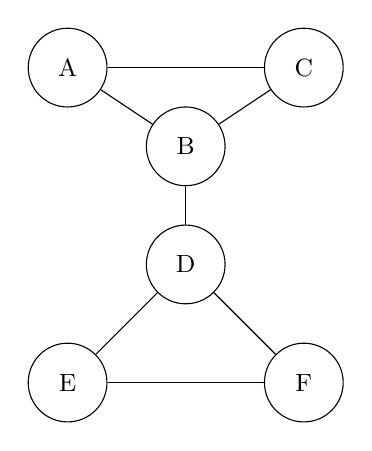
\begin{tikzpicture}[every node/.style={circle,draw,minimum size=10mm,inner sep=1pt}, font=\small]
			
			% Vertices
			\node (A) at (0,2) {A};
			\node (B) at (1.5,1) {B};
			\node (C) at (3,2) {C};
			\node (D) at (1.5,-0.5) {D};
			\node (E) at (0,-2) {E};
			\node (F) at (3,-2) {F};
			
			% Edges
			\draw (A) -- (B);
			\draw (B) -- (C);
			\draw (A) -- (C);
			\draw (B) -- (D);
			\draw (D) -- (E);
			\draw (D) -- (F);
			\draw (E) -- (F);
			
		\end{tikzpicture}
		\caption{Undirected graph for articulation point detection}
	\end{figure}
	
	\begin{figure}[H]
		\centering
		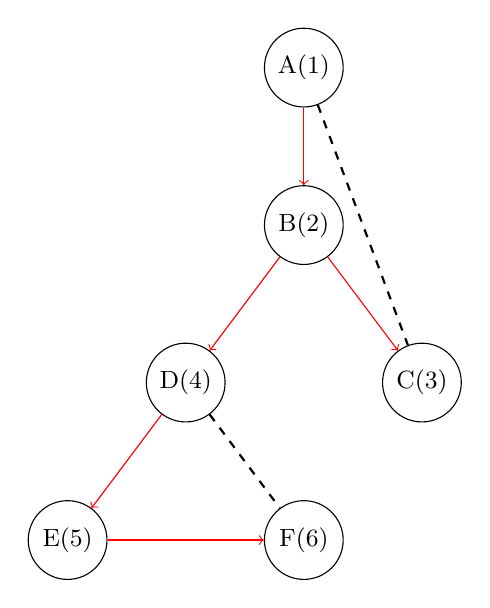
\begin{tikzpicture}[every node/.style={circle,draw,minimum size=10mm,inner sep=1pt}, font=\small]
			
			% Nodes with (DFS, Low) labels
			\node (1) at (0,4) {A(1)};
			\node (2) at (0,2) {B(2)};
			\node (3) at (1.5,0) {C(3)};
			\node (4) at (-1.5,0) {D(4)};
			\node (5) at (-3,-2) {E(5)};
			\node (6) at (0,-2) {F(6)};
			
			% Tree edges (red arrows)
			\draw[red, ->] (1) -- (2);
			\draw[red, ->] (2) -- (3);
			\draw[red, ->] (2) -- (4);
			\draw[red, ->] (4) -- (5);
			\draw[red, ->] (5) -- (6);
			
			% Back edges (black dashed)
			\draw[black, thick, dashed] (1) -- (3);
			\draw[black, thick, dashed] (4) -- (6);
			
		\end{tikzpicture}
		\caption{DFS tree of the graph}
	\end{figure}
	
	\subsection*{Steps of DFS and articulation point calculation}
	
	We start the DFS from vertex \(A\). The following table shows the DFNum and Low values for each vertex.
	
	\begin{table}[H]
		\centering
		\begin{adjustbox}{center}
			\begin{tabular}{|c|c|c|}
				\hline
				Vertex & DFNum & Low \\
				\hline
				A & 1 & 1 \\
				\hline
				B & 2 & 1 \\
				\hline
				C & 3 & 1 \\
				\hline
				D & 4 & 4 \\
				\hline
				E & 5 & 4 \\
				\hline
				F & 6 & 4 \\
				\hline
			\end{tabular}
		\end{adjustbox}
		\caption{DFNum and Low values for each vertex}
	\end{table}
	
	Using the Low values and the articulation point rules:
	\begin{itemize}
		\item If a child \(v\) of \(u\) satisfies \(\text{Low}[v] \ge \text{DFNum}[u]\), then \(u\) is an articulation point (except for the root).
		\item The root is an articulation point if it has more than one child in the DFS tree.
	\end{itemize}
	
	The set of articulation points in this graph is:
	\[
	\{B,\ D\}
	\]
	
	\section{Conclusion}
	
	Using the DFS algorithm and correctly computing the values of \(\EN{DFNum}\) and \(\EN{Low}\), we can identify articulation points. In the example above, removing \(B\) disconnects the subtree containing \(E\), and removing \(D\) disconnects its child subtrees. Thus \(B\) and \(D\) are articulation points.
	
\end{document}